\chapter{Computational details}
\label{sec:Computation}

\section{Settings and dependencies}

The calculations in this project was enabled from allocated resources on the supercomputer FRAM of Uninett Sigma2 \textbf{add citation}, utilizing the Vienna Ab initio Simulation Package (VASP) \textbf{add citation}. As discussed the caluclations employed the projector-augmented-wave method and PBE GGA in addition to SCAN meta-GGA and HSE06 in relevant cases. For the structures studied in this project we found an energy cutoff of 300 eV and 400 eV suitable for electronic and geometric relaxations respectively. In regards to the number of k-points we used a gamma centered mesh with density of 4 \si{\angstrom}. The geometric relaxation of ionic positions and cell volume was carried out in two subsequent runs with convergence criterion of \num{1E-2} for the forces and \num{1E-5} for the total energy, with Gaussian smearing (ISMEAR = 0 in VASP) and smearing width $\sigma$ equal to 0.05 eV. After successful geometric relaxation the structures underwent a final electronic relaxation with the tetrahedron method with Bloch corrections (TBC, ISMEAR = -5 in VASP) and a energy criterion of \num{1E-6}. Magnetic materials was handled with the setting ISPIN = 2 in VASP which perform co-linear spin-polarized calculations, further customization of the magnetic configurations was beyond the scope of this project. 

The hybrid functional HSE06 proved challenging to converge, to solve the convergence problem we reduced the density of k-points from 4 \si{\angstrom} to 2 \si{\angstrom} and performed calculations first with Gaussian smearing ($\sigma = 0.05$) and reapplied the calculated charge density to perform a subsequent calculation with TBC.

The special quasi-random structures method was implemented through the generate$\-$structure script in the \textit{Temperature dependent effective potential} (TDEP) package \textbf{add citation}. Cif-files for the relevant structures was obtained from Materials project \cite{Jain2013}. To simplify both the work-flow of the project and extract relevant data we utilized tools from  from the python library pymatgen, and vaspkit package \textbf{citation?} In addition to several utility scripts was both devolped during the project and provided by SINTEF, these can be found at ..\textbf{insert github address.}


\section{Material}

\begin{figure}[H]
\begin{subfigure}{0.5\textwidth}
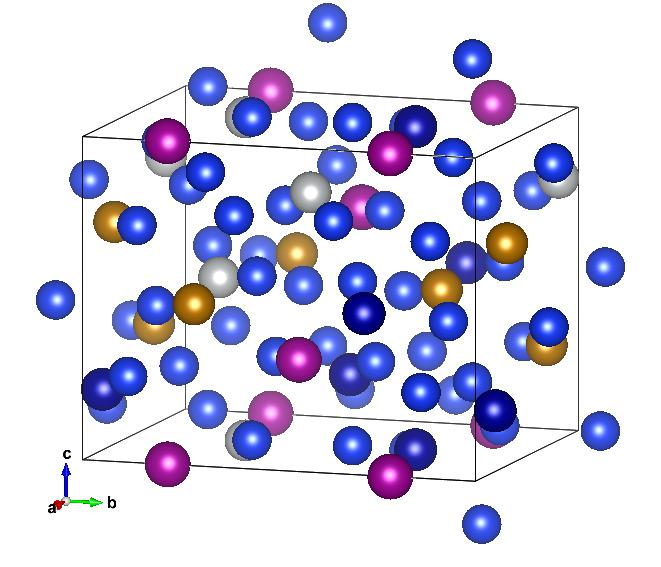
\includegraphics[width=\textwidth]{method/sqs/A.jpg}
\caption{A}
\end{subfigure}
\hfill
\begin{subfigure}{0.5\textwidth}
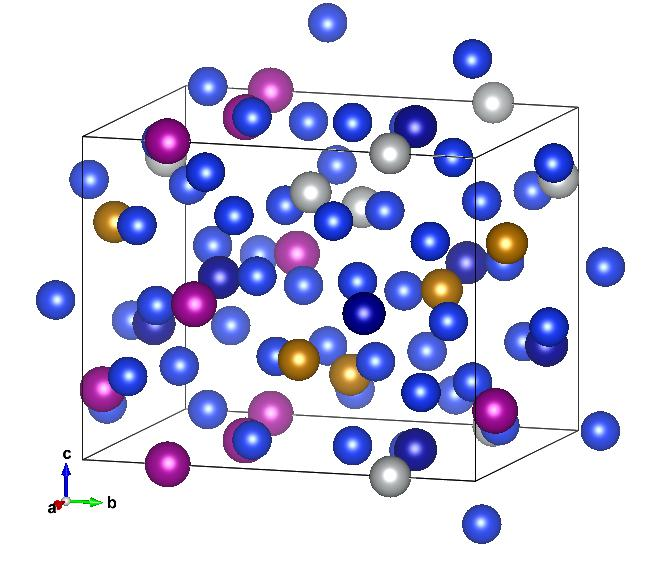
\includegraphics[width=\textwidth]{method/sqs/B.jpg}
\caption{B}
\end{subfigure}
\begin{subfigure}{0.5\textwidth}
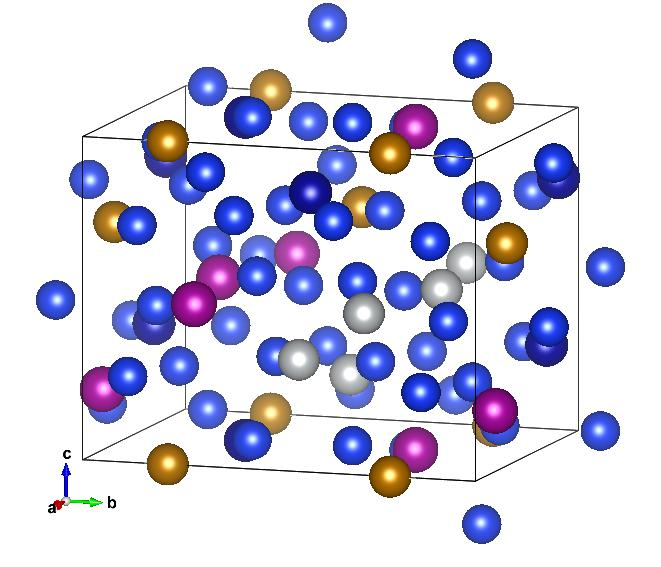
\includegraphics[width=\textwidth]{method/sqs/C.jpg}
\caption{C}
\end{subfigure}
\hfill
\begin{subfigure}{0.5\textwidth}
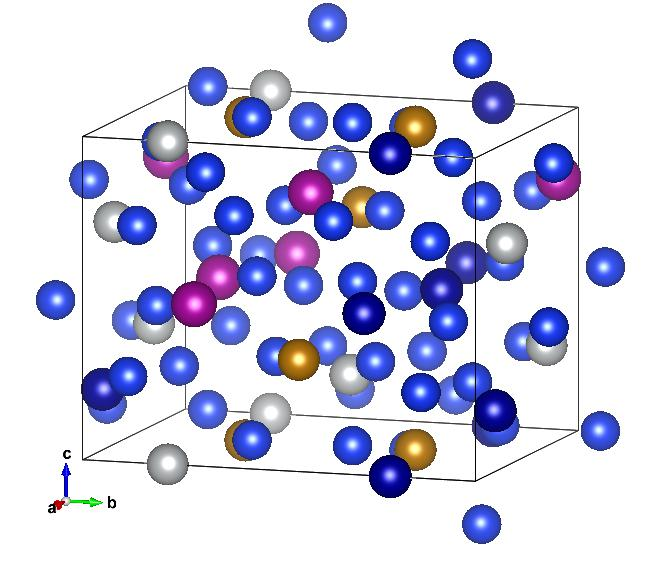
\includegraphics[width=\textwidth]{method/sqs/D.jpg}
\caption{D}
\end{subfigure}
\begin{subfigure}{0.5\textwidth}
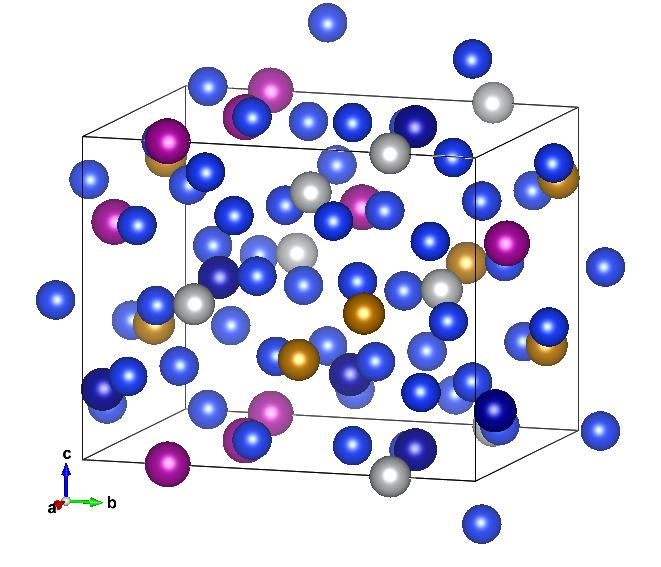
\includegraphics[width=\textwidth]{method/sqs/E.jpg}
\caption{E}
\end{subfigure}
\caption{5 distinct 48 atom SQS of \ch{Cr4Fe4Mn4Ni4Si32} based on the $\beta-$ \ch{FeSi2} crystal structure. Illustrated with VESTA \cite{vesta}}
\label{sqs_FeSi2}
\end{figure}

In this project we have constructed high-entropy silicides based on the $\beta-$ \ch{FeSi2} compound. The unit cell of this material is in the orthogonal cmce crystal lattice, and consists of 16 iron atoms and 32 silicon atoms. Per composition we generate 5 distinct SQSs of equivalent geometry and composition that only vary by atomic configuration. We have emphasized a particular composition of the 3d elements Cr, Fe, Mn, and Ni in a \ch{Cr4Fe4Mn4Ni4Si32} alloy where the 3d elements are distributed equimolarly and occupy the Fe-sites in the $\beta-$ \ch{FeSi2} crystal structure. These SQSs can be seen in figure 6.1 where manganese atoms are represented as purple spheres, chromium as dark blue and silicon as light blue, followed by iron and nickel presented as gold and silver spheres respectively. The respective SQSs are denoted as A, B, C, D and E. In addition to the \ch{(CrFeMnNi)Si2} composition we have trialed other compositions with varying distribution and elements generated by an identical procedure consistent with the 48 atom SQS model.
